\documentclass[11pt]{article}\usepackage[]{graphicx}\usepackage[]{color}
%% maxwidth is the original width if it is less than linewidth
%% otherwise use linewidth (to make sure the graphics do not exceed the margin)
\makeatletter
\def\maxwidth{ %
  \ifdim\Gin@nat@width>\linewidth
    \linewidth
  \else
    \Gin@nat@width
  \fi
}
\makeatother

\definecolor{fgcolor}{rgb}{0, 0, 0}
\newcommand{\hlnum}[1]{\textcolor[rgb]{0,0,0}{#1}}%
\newcommand{\hlstr}[1]{\textcolor[rgb]{0,0,0}{#1}}%
\newcommand{\hlcom}[1]{\textcolor[rgb]{0.4,0.4,0.4}{\textit{#1}}}%
\newcommand{\hlopt}[1]{\textcolor[rgb]{0,0,0}{\textbf{#1}}}%
\newcommand{\hlstd}[1]{\textcolor[rgb]{0,0,0}{#1}}%
\newcommand{\hlkwa}[1]{\textcolor[rgb]{0,0,0}{\textbf{#1}}}%
\newcommand{\hlkwb}[1]{\textcolor[rgb]{0,0,0}{\textbf{#1}}}%
\newcommand{\hlkwc}[1]{\textcolor[rgb]{0,0,0}{\textbf{#1}}}%
\newcommand{\hlkwd}[1]{\textcolor[rgb]{0,0,0}{\textbf{#1}}}%
\let\hlipl\hlkwb

\usepackage{framed}
\makeatletter
\newenvironment{kframe}{%
 \def\at@end@of@kframe{}%
 \ifinner\ifhmode%
  \def\at@end@of@kframe{\end{minipage}}%
  \begin{minipage}{\columnwidth}%
 \fi\fi%
 \def\FrameCommand##1{\hskip\@totalleftmargin \hskip-\fboxsep
 \colorbox{shadecolor}{##1}\hskip-\fboxsep
     % There is no \\@totalrightmargin, so:
     \hskip-\linewidth \hskip-\@totalleftmargin \hskip\columnwidth}%
 \MakeFramed {\advance\hsize-\width
   \@totalleftmargin\z@ \linewidth\hsize
   \@setminipage}}%
 {\par\unskip\endMakeFramed%
 \at@end@of@kframe}
\makeatother

\definecolor{shadecolor}{rgb}{.97, .97, .97}
\definecolor{messagecolor}{rgb}{0, 0, 0}
\definecolor{warningcolor}{rgb}{1, 0, 1}
\definecolor{errorcolor}{rgb}{1, 0, 0}
\newenvironment{knitrout}{}{} % an empty environment to be redefined in TeX

\usepackage{alltt}
\usepackage{fullpage,graphicx,float,amsmath,enumitem,hyperref}
\setlist{parsep=5.5pt}
\setlength{\parindent}{0pt}
\setlength{\parskip}{\baselineskip}

\usepackage{fancyhdr}
\pagestyle{fancy}
\lhead{Time Series HW 8}
\rhead{Allison Theobold, Andrea Mack, and Kenny Flagg}
\setlength{\headheight}{18pt}
\setlength{\headsep}{2pt}

\title{Time Series HW 8}
\author{Allison Theobold, Andrea Mack, and Kenny Flagg}
\date{November 29, 2016}
\IfFileExists{upquote.sty}{\usepackage{upquote}}{}
\begin{document}
\maketitle




Volatility occurs when the conditional variance of a time series varies over time (CC, 279).



The ACF and PACF of the daily returns both suggest statistically significant autocorrelation at lags 1, 4, and 5. 

\begin{knitrout}\footnotesize
\definecolor{shadecolor}{rgb}{1, 1, 1}\color{fgcolor}

{\centering 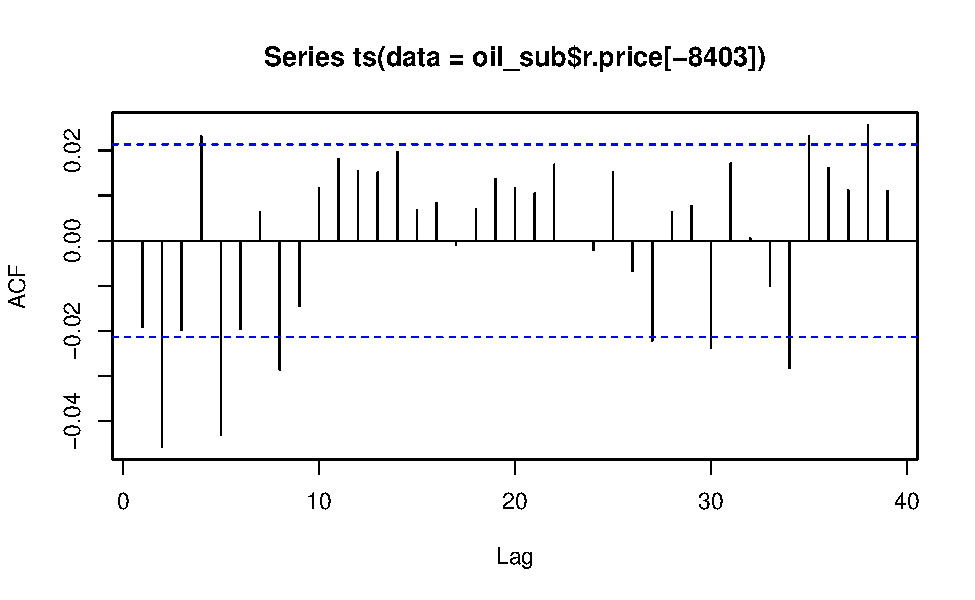
\includegraphics[width=\maxwidth]{figure/assess_autocorr-1} 

}




{\centering 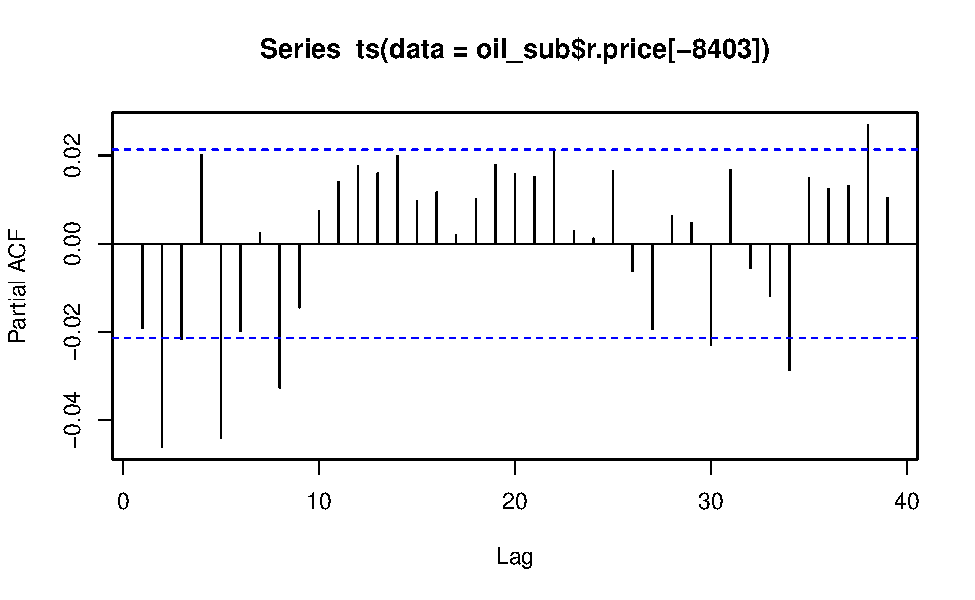
\includegraphics[width=\maxwidth]{figure/assess_autocorr-2} 

}




{\centering 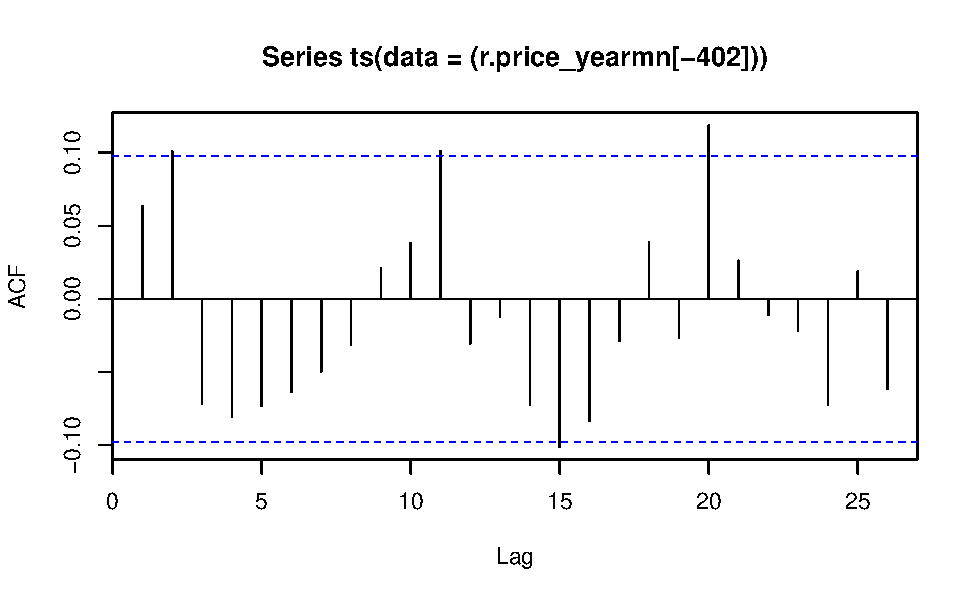
\includegraphics[width=\maxwidth]{figure/assess_autocorr-3} 

}




{\centering 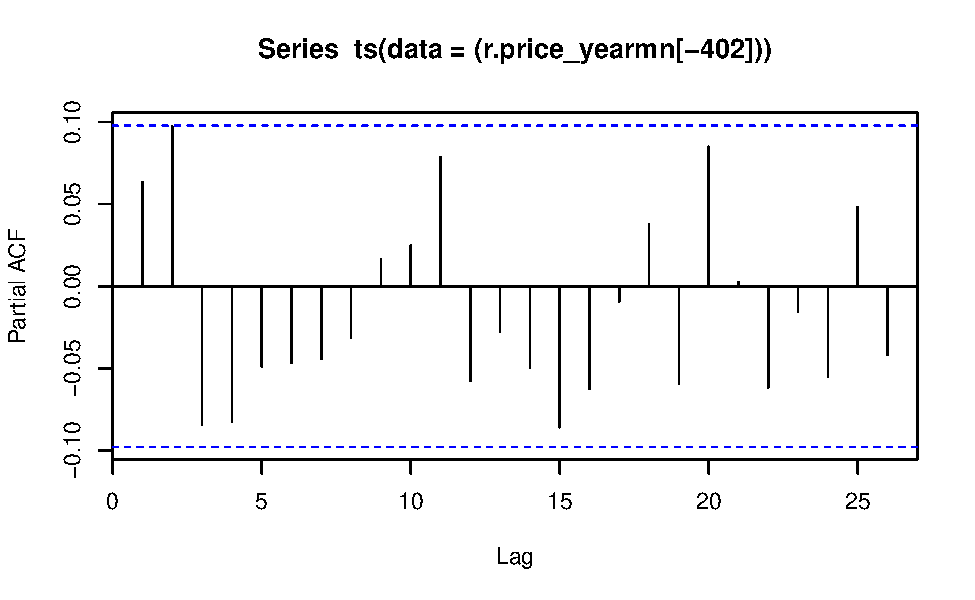
\includegraphics[width=\maxwidth]{figure/assess_autocorr-4} 

}



\end{knitrout}

To determine whether observations are independent and identically distributed, versus just having correlated observations, look at the ACF and PACF of the absolute value of the responses (CC 281). There is strong evidence monthly log price returns are not independent and identically distributed. 

Idea: if lags in ts are independent, then independence will hold through (even) non-linear transformations, whereas if they are uncorrelated, *un*correlation will only hold through linear transformations.

\begin{knitrout}\footnotesize
\definecolor{shadecolor}{rgb}{1, 1, 1}\color{fgcolor}

{\centering 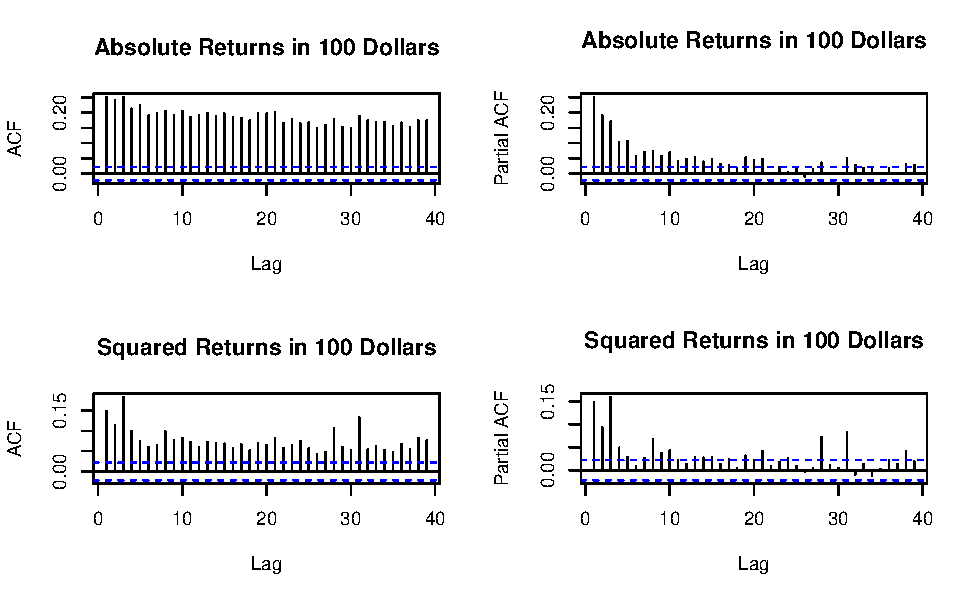
\includegraphics[width=\maxwidth]{figure/abs_plots-1} 

}




{\centering 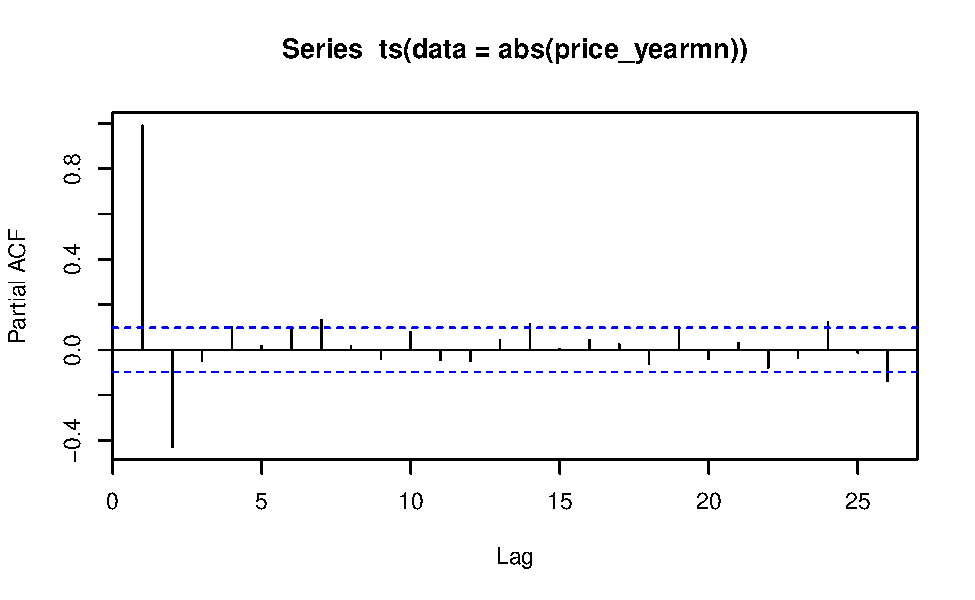
\includegraphics[width=\maxwidth]{figure/abs_plots-2} 

}




{\centering 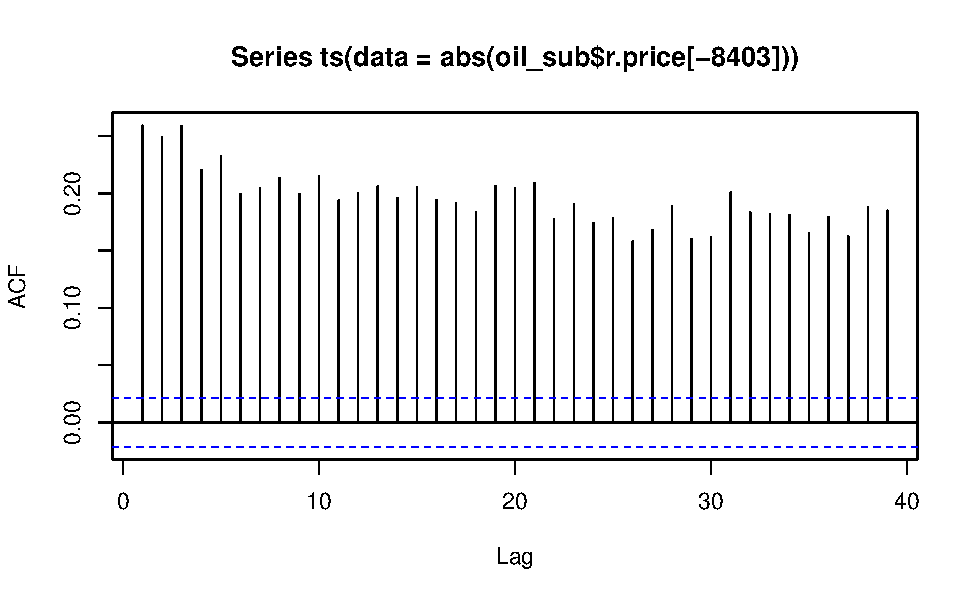
\includegraphics[width=\maxwidth]{figure/abs_plots-3} 

}




{\centering 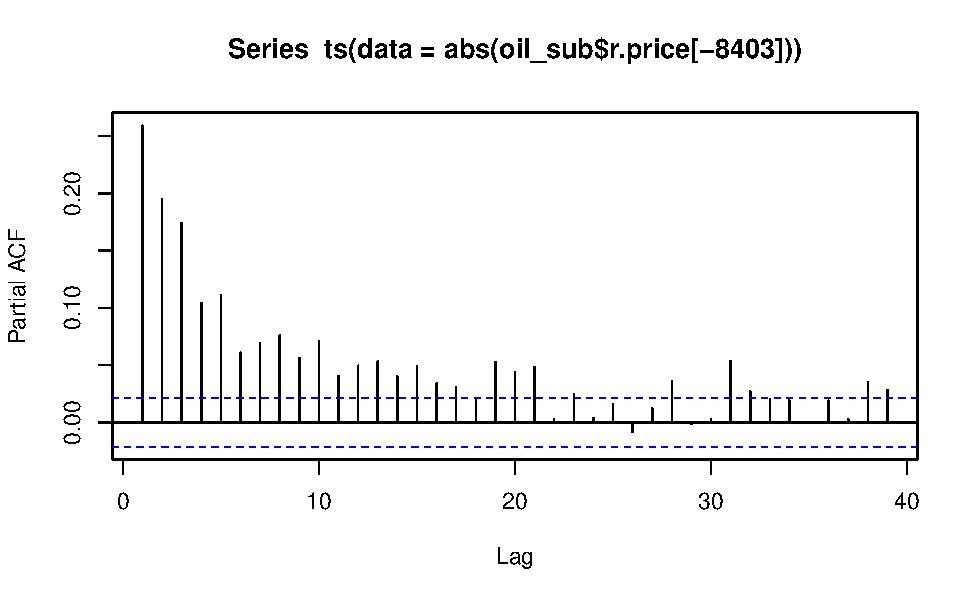
\includegraphics[width=\maxwidth]{figure/abs_plots-4} 

}




{\centering 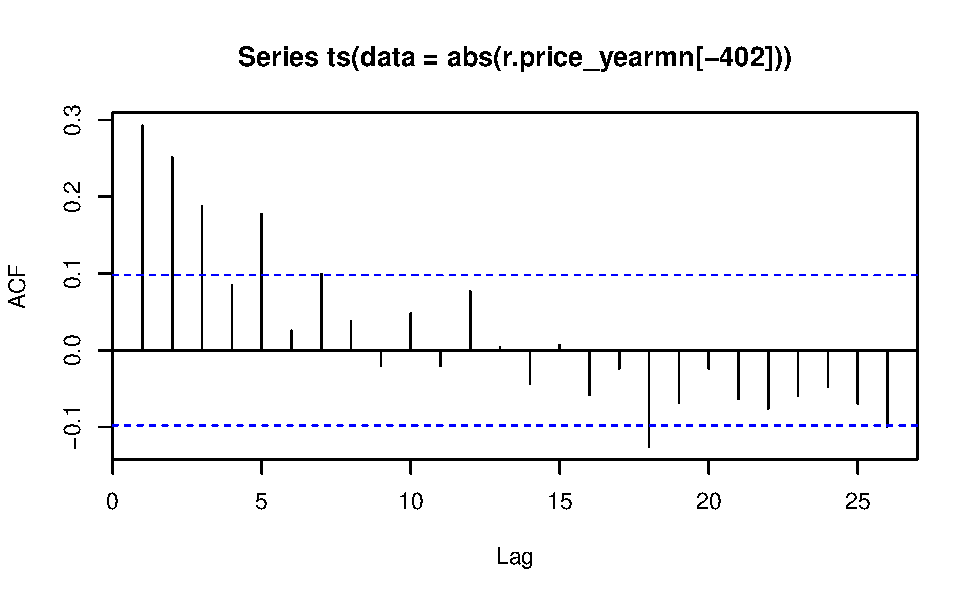
\includegraphics[width=\maxwidth]{figure/abs_plots-5} 

}




{\centering 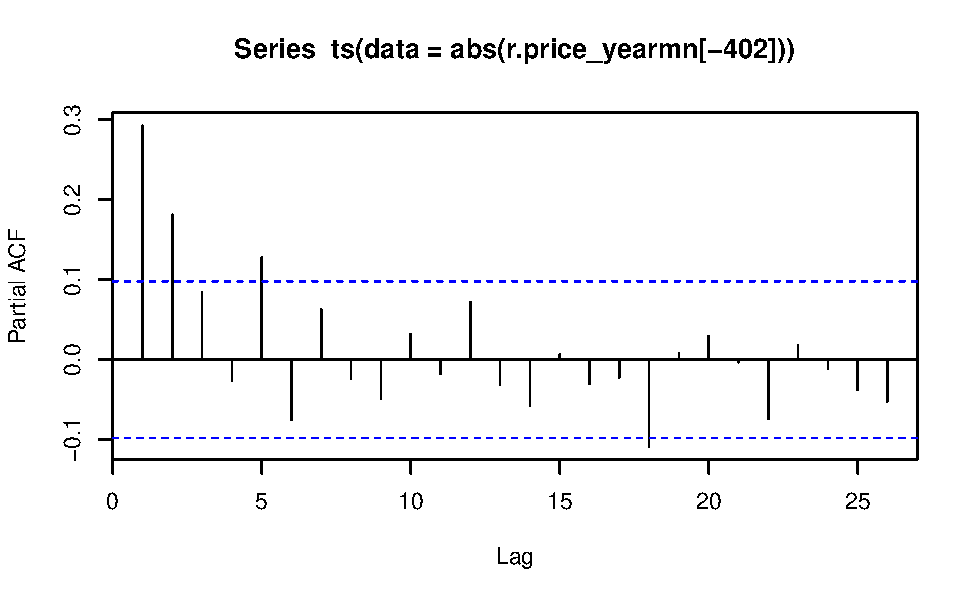
\includegraphics[width=\maxwidth]{figure/abs_plots-6} 

}




{\centering 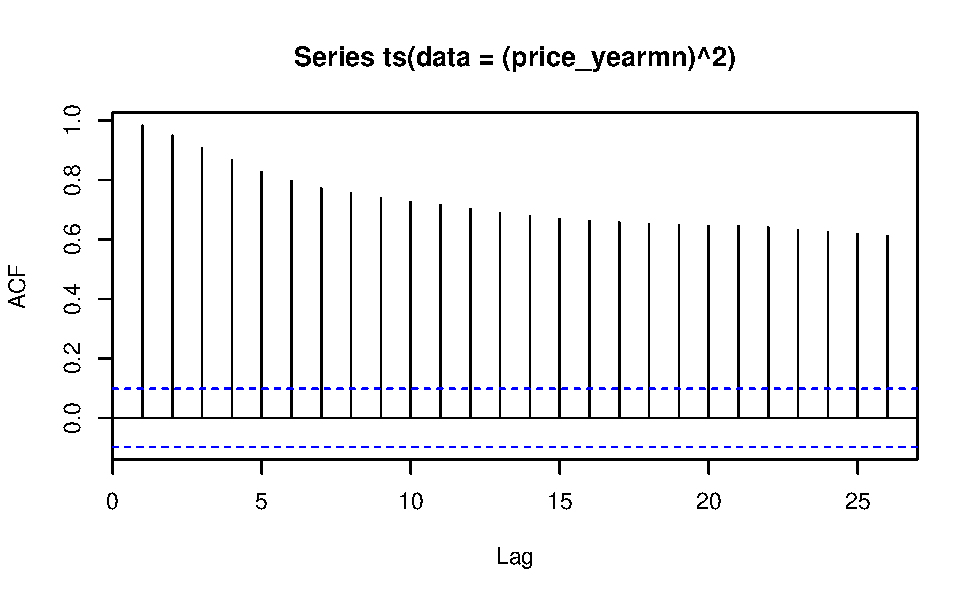
\includegraphics[width=\maxwidth]{figure/abs_plots-7} 

}




{\centering 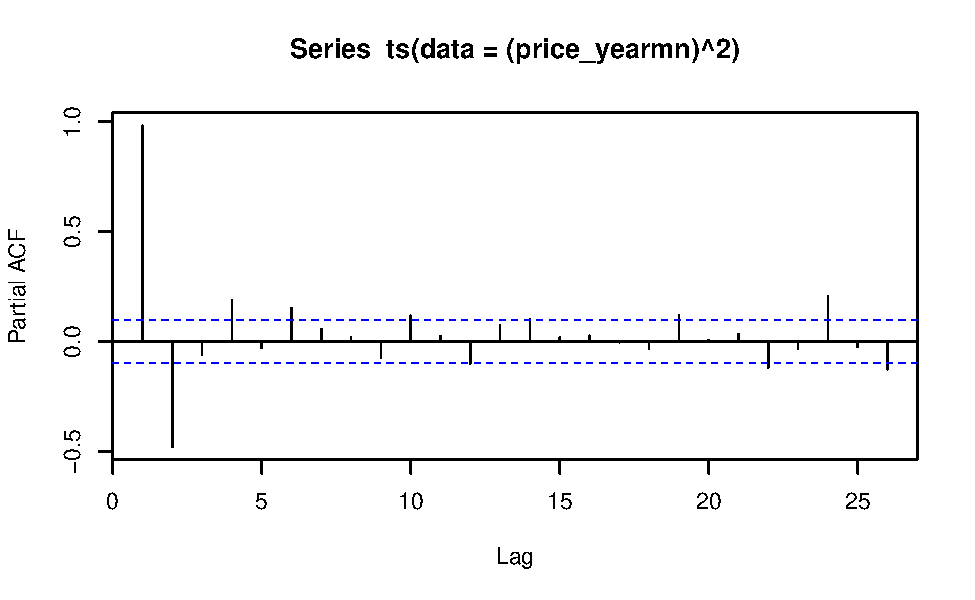
\includegraphics[width=\maxwidth]{figure/abs_plots-8} 

}




{\centering 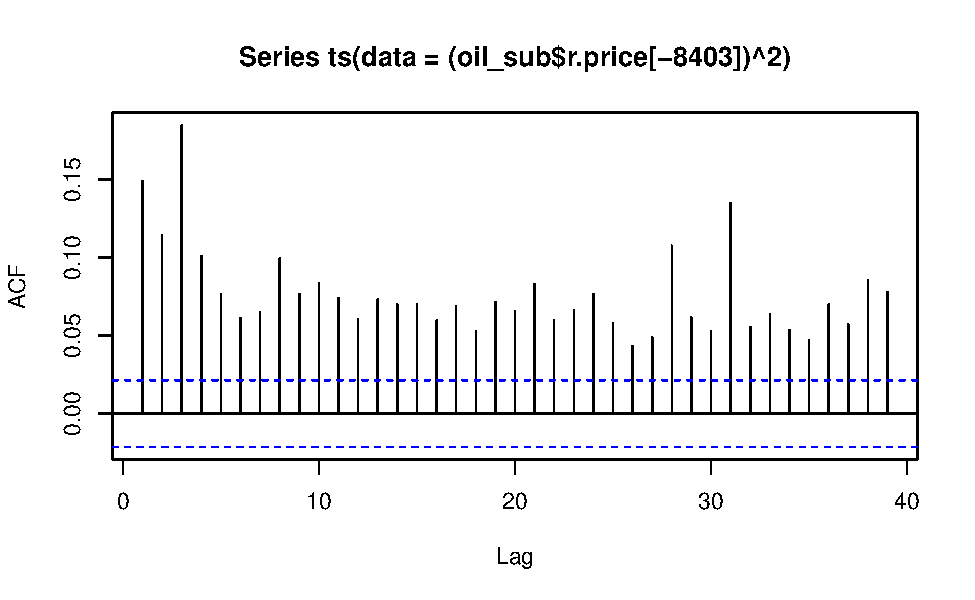
\includegraphics[width=\maxwidth]{figure/abs_plots-9} 

}




{\centering 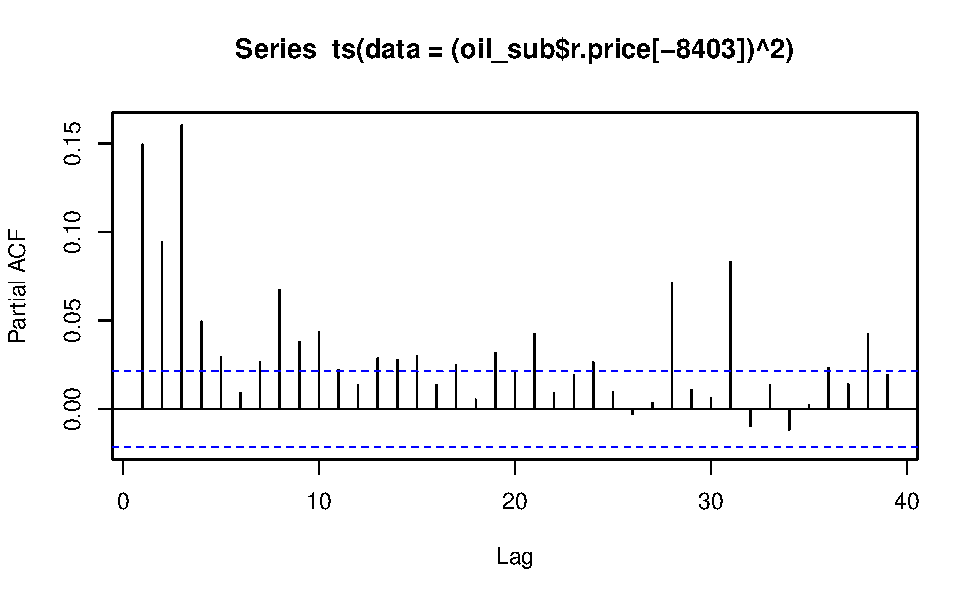
\includegraphics[width=\maxwidth]{figure/abs_plots-10} 

}




{\centering 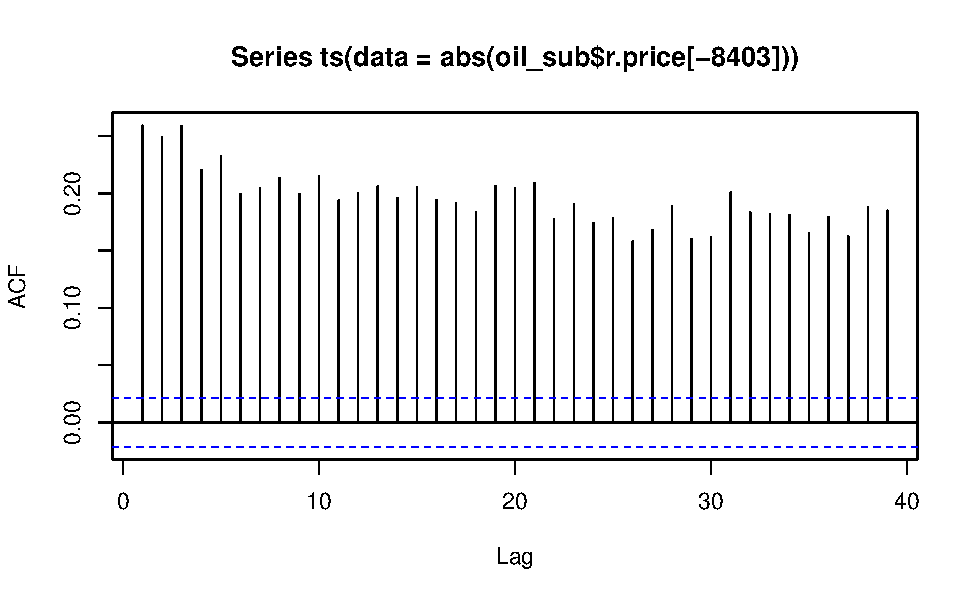
\includegraphics[width=\maxwidth]{figure/abs_plots-11} 

}




{\centering 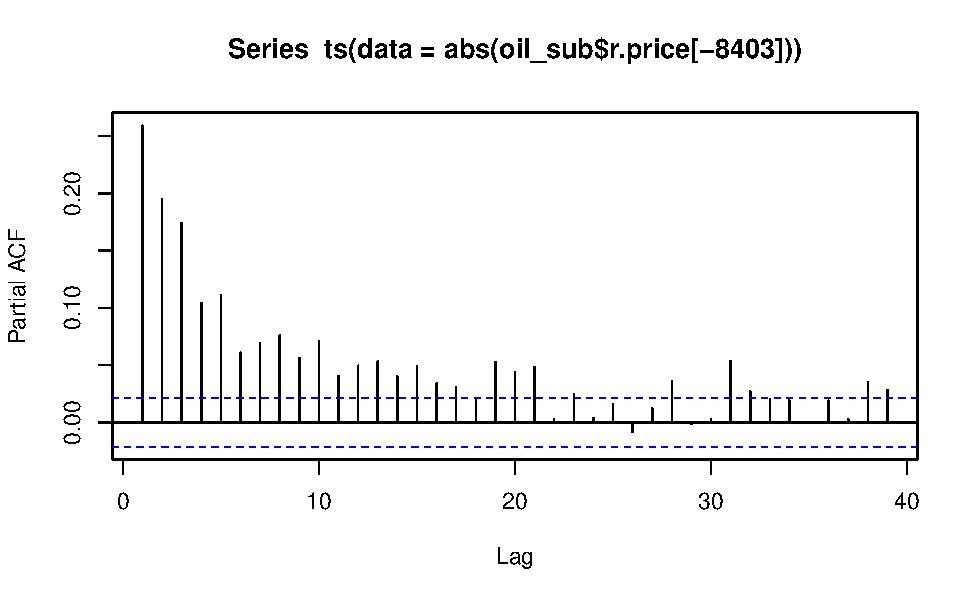
\includegraphics[width=\maxwidth]{figure/abs_plots-12} 

}




{\centering 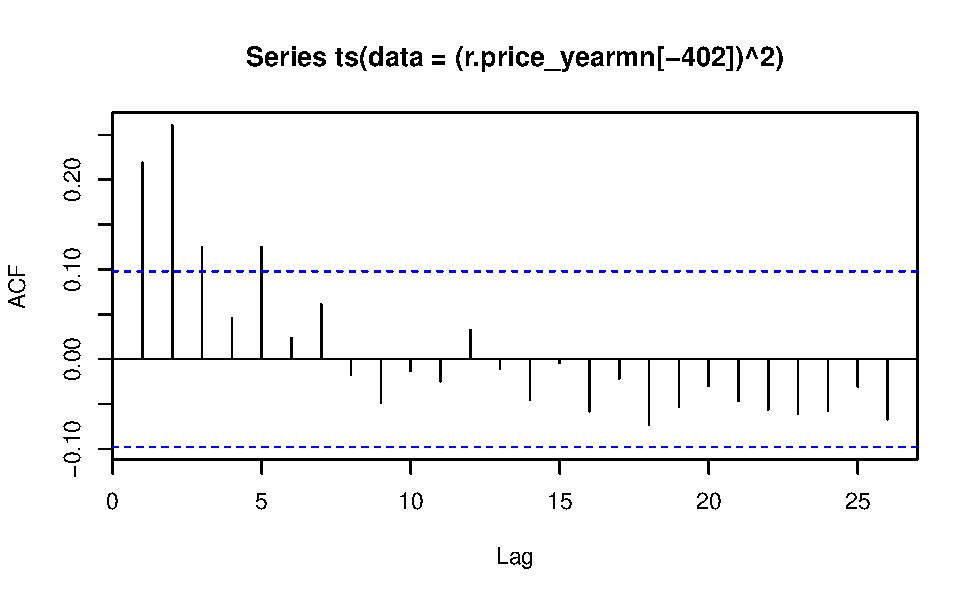
\includegraphics[width=\maxwidth]{figure/abs_plots-13} 

}




{\centering 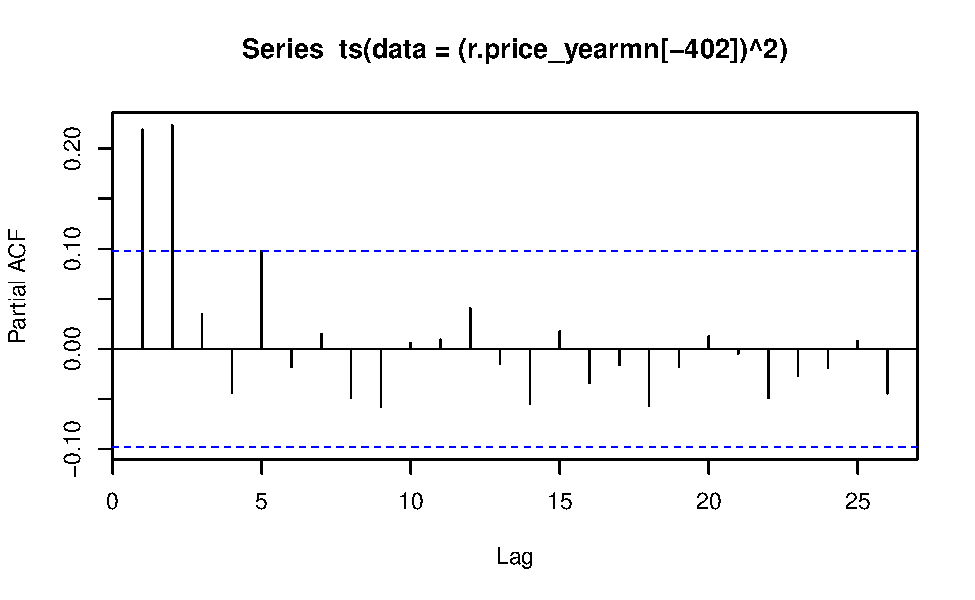
\includegraphics[width=\maxwidth]{figure/abs_plots-14} 

}




{\centering 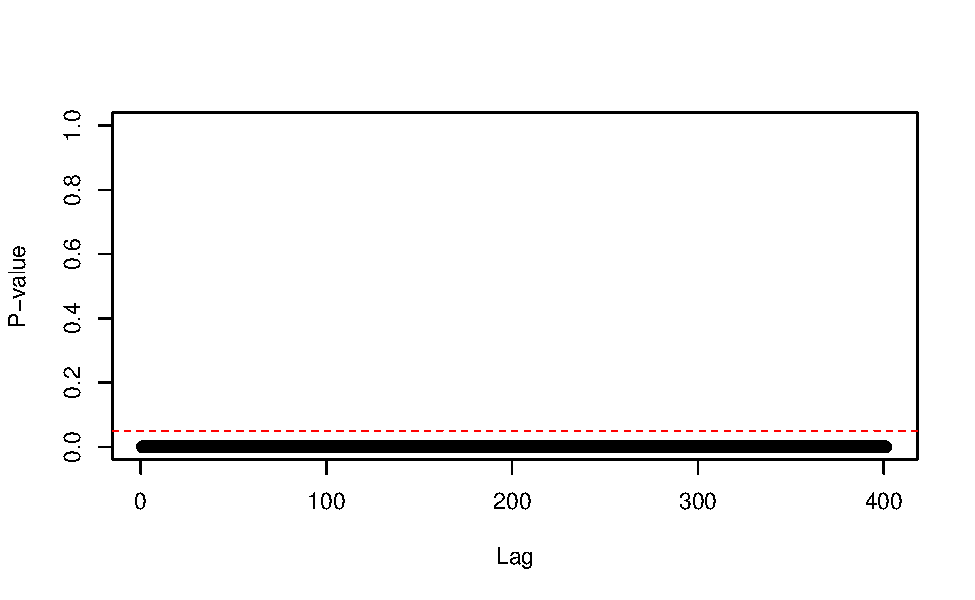
\includegraphics[width=\maxwidth]{figure/abs_plots-15} 

}




{\centering 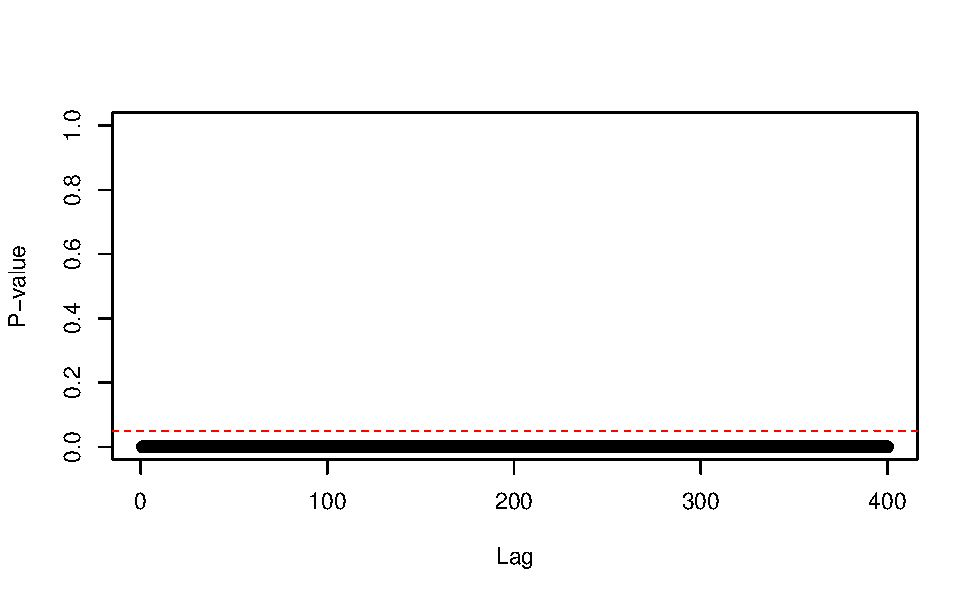
\includegraphics[width=\maxwidth]{figure/abs_plots-16} 

}



\end{knitrout}


Box-Ljung/McLeod-Li test

$H_{o}$: no ARCH

$H_{a}$: ARCH

Both the monthly and daily prices as well as the returns suggest strong evidence of ARCH at all lags.

\begin{knitrout}\footnotesize
\definecolor{shadecolor}{rgb}{1, 1, 1}\color{fgcolor}

{\centering 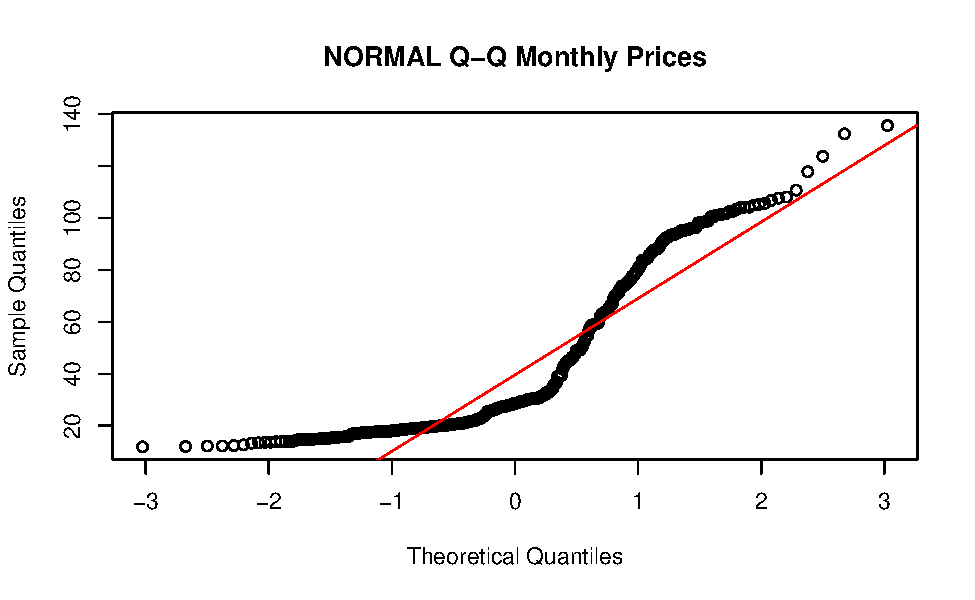
\includegraphics[width=\maxwidth]{figure/norm-1} 

}




{\centering 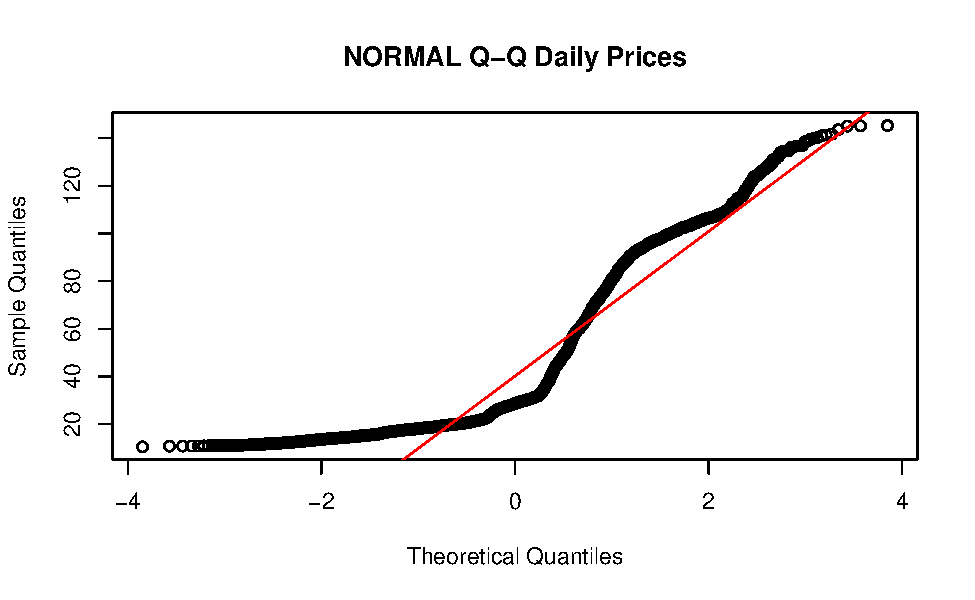
\includegraphics[width=\maxwidth]{figure/norm-2} 

}




{\centering 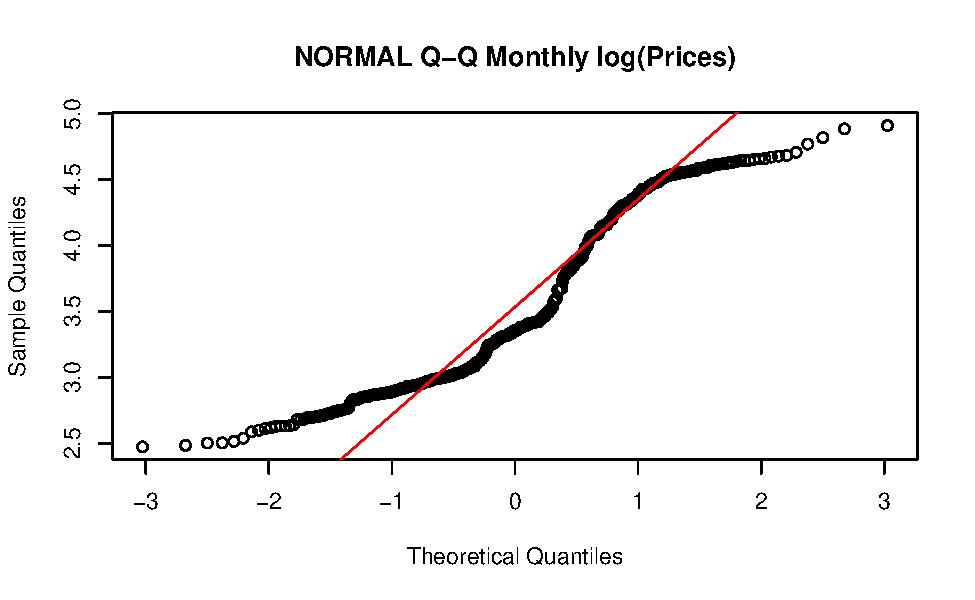
\includegraphics[width=\maxwidth]{figure/norm-3} 

}




{\centering 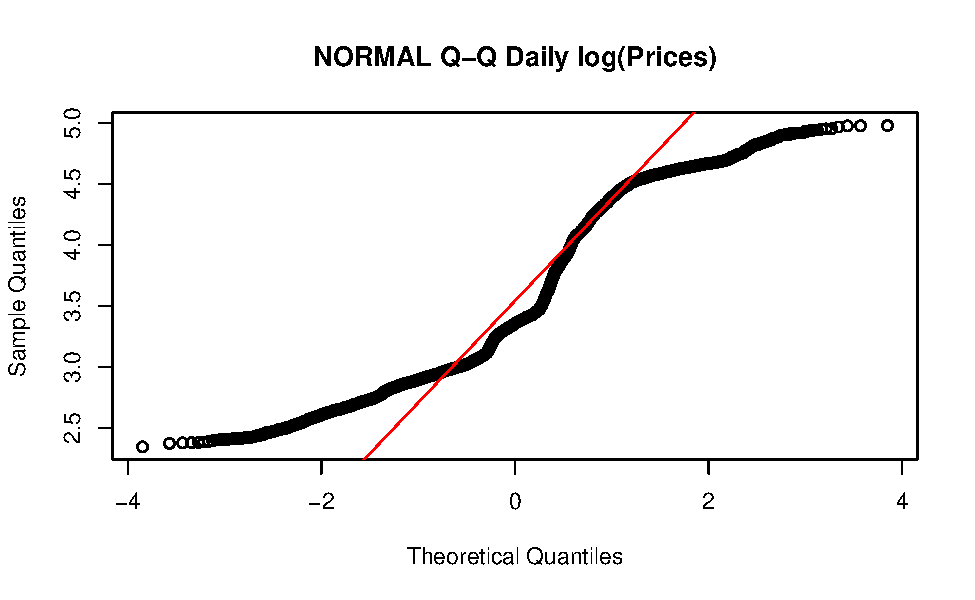
\includegraphics[width=\maxwidth]{figure/norm-4} 

}




{\centering 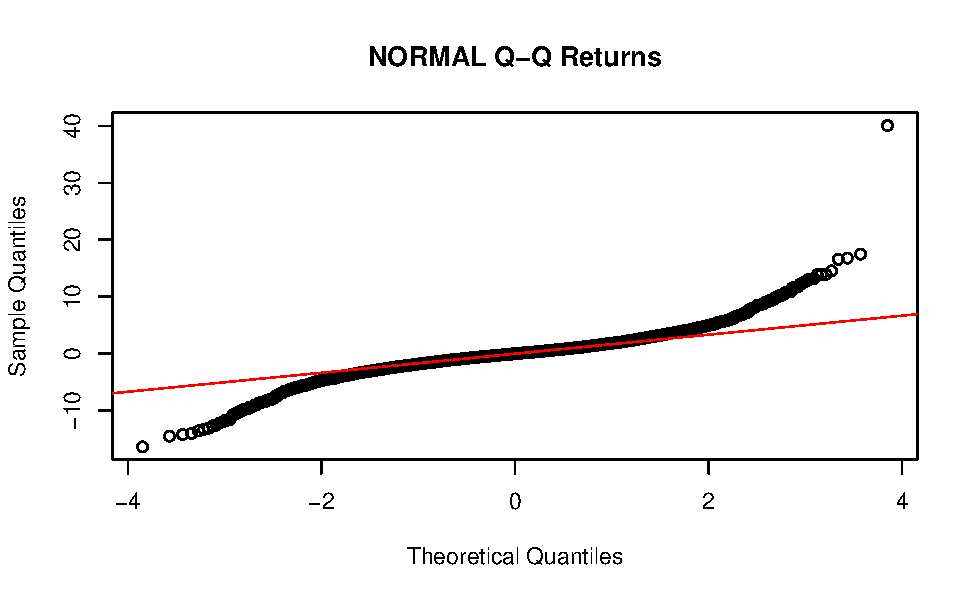
\includegraphics[width=\maxwidth]{figure/norm-5} 

}



\end{knitrout}

The return($r_{t}$) in financial time series is defined by CC as:

$r_{t} = log(price_{t}) - log(price_{t-1})$

The return is thus define as the ratio of the log prices between two subsequent time points. The return is often then scaled by 100 to make numbers more easily thought about. The ACF and PACF of the returns suggest significant autocorrelations at the 5\% significance level. The ACF and PACF of the absolute value and squared returns both suggest independence is violated. Non-significant autocorrelation and signficiant violations of independence are commmon suggest volatility clustering. Volatility clustering visually is seen when the returns closer together display more similar variability. The Normal Q-Q plot of the returns shows heavy tails. Heavy tailed distributions and volatitlity clustering are common in financial time series data (CC 285). ARCH and GARCH models are used when data display these characteristics. 

Let the conditional variance of the returns, Var($r_{t|t-1}$) = $\sigma_{t|t-1}$. In ARCH modeling, a linear regression model of order q is fit to describe the relationship between the current conditional variance and the previous returns. 

$r_{t} = \sigma_{t|t-q}\epsilon_{t}$

$\sigma^{2}_{t|t-q} = \omega + \Sigma_{i=1:q} \alpha_{i}r^{2}_{t-i}$

such that $\epsilon_{t} \sim (0,1)$ and $\epsilon_{t} \perp r_{t-j}$ for j = 1,2,...

The conditional variance is not observable, and so with a linear transformation, the current squared return can be transformed to be a linear combination of previous squared returns and a random error such that

$\r^{2}_{t} = \omega + \Sigma_{i=1:q} \alpha_{i}r^{2}_{t-i} + \Nu_{t}$

which is the form of an AR(q) process. 





\end{document}
